%% This is file `DEMO-TUDaExercise.tex' version 2.09 (2020/03/13),
%% it is part of
%% TUDa-CI -- Corporate Design for TU Darmstadt
%% ----------------------------------------------------------------------------
%%
%%  Copyright (C) 2018--2020 by Marei Peischl <marei@peitex.de>
%%
%% ============================================================================
%% This work may be distributed and/or modified under the
%% conditions of the LaTeX Project Public License, either version 1.3c
%% of this license or (at your option) any later version.
%% The latest version of this license is in
%% http://www.latex-project.org/lppl.txt
%% and version 1.3c or later is part of all distributions of LaTeX
%% version 2008/05/04 or later.
%%
%% This work has the LPPL maintenance status `maintained'.
%%
%% The Current Maintainers of this work are
%%   Marei Peischl <tuda-ci@peitex.de>
%%   Markus Lazanowski <latex@ce.tu-darmstadt.de>
%%
%% The development respository can be found at
%% https://github.com/tudace/tuda_latex_templates
%% Please use the issue tracker for feedback!
%%
%% ============================================================================
%%
% !TeX program = lualatex
%%

\documentclass[
	ngerman,
     solution=true
	]{tudaexercise}

\usepackage{verbatim}
\usepackage[english, main=ngerman]{babel}
\usepackage[babel]{csquotes}

\usepackage{biblatex}
\usepackage{amsmath}
\usepackage{ulem}
\usepackage{arydshln}
\usepackage{amsfonts}
\usepackage{listings}
\usepackage{color}
\usepackage{geometry}
\usepackage{graphicx} 
\usepackage{float} 
\usepackage{subfigure}
\definecolor{dkgreen}{rgb}{0,0.6,0}
\definecolor{gray}{rgb}{0.5,0.5,0.5}
\definecolor{mauve}{rgb}{0.58,0,0.82}

\lstset{frame=tb,
  language=Python,
  aboveskip=3mm,
  belowskip=3mm,
  showstringspaces=false,
  columns=flexible,
  basicstyle={\small\ttfamily},
  numbers=none,
  numberstyle=\tiny\color{gray},
  keywordstyle=\color{blue},
  commentstyle=\color{dkgreen},
  stringstyle=\color{mauve},
  breaklines=true,
  breakatwhitespace=true,
  tabsize=3
}
\bibliography{DEMO-TUDaBibliography}

%Formatierungen für Beispiele in diesem Dokument. Im Allgemeinen nicht notwendig!
\let\file\texttt
\let\code\texttt
\let\pck\textsf
\let\cls\textsf
\let\tbs\textbackslash

\ConfigureHeadline{
	headline={title-name-id}
}

%compatbilitx
\let\unit\relax

\begin{document}

\title[Übung TUDaExercise]{Statistical Machine Learning:\\Exercise$\quad$3}
\author{Yi Cui,2758172\\ Lingwei Liu,2659255}
\term{Sommersemester 2020}
%\sheetnumber{5}

\maketitle

\begin{task}{Linear Regression}
In this exercise, you will implement various kinds of linear regression using the data lin\_reg\_train.txt and
 lin\_reg\_test.txt. The files contain noisy observations from an unknown function $ f: \mathbb{R} \mapsto \mathbb{R}$ In both files,
the first column represents the inputs and the second column represents the outputs. You can load the data using
numpy.loadtxt.
For all subtasks, assume that the data is identically and independently distributed according to
\[
y_{i}=\boldsymbol{\Phi}\left(\mathbf{x}_{\mathbf{i}}\right)^{\top} \mathbf{w}+\epsilon_{i} ,
\]
where
\[
\epsilon_{i} \sim \mathcal{N}\left(0, \sigma^{2}\right)
\]
and $ \Phi: \mathbb{R}^{1} \rightarrow \mathbb{R}^{n}$ is a feature transformation such that
\[
\mathbf{y} \sim \mathcal{N}\left(\mathbf{\Phi}(\mathbf{X})^{\top} \mathbf{w}, \sigma^{2} \mathbf{I}\right)
\]
Additionally, make sure that your implementations support multivariate inputs. The feature transformation are given
in each task, if no basis functions are stated explicitely use the data as is $\Phi(x) = x$.


%--------------------------------------------------------------------------------------------------1a---------------------------------------------------------------------------------------
\begin{subtask}[1a)]
Implement linear ridge regression using linear features, i.e. the data itself. Include an additional input dimension to
represent a bias term and use the ridge coefficient $ \mu = 0.01$.\\[15pt]
1. Explain: What is the ridge coefficient and why do we use it? (1)\\[15pt]
2. Derive the optimal model parameters by minimizing the squared error loss function. (3)\\[15pt]
3. Report the root mean squared error of the train and test data under your linear model with linear features. (2)\\[15pt]
4. Include a single plot that shows the training data as black dots and the predicted function as a blue line. (2)
%%
\\[15pt]
answer:\\[15pt]
ridge coefficient lambda in
\[
\mathbf{w}_{\mathrm{MAP}}=\left(\Phi \Phi^{\mathrm{T}}+\frac{\alpha}{\beta} \mathbf{1}\right)^{-1} \Phi \mathbf{y}
\]
reason: regularizes the pseudo-inverse\\
root mean squared error of the training data: 2.9145386993882525\\
root mean squared error of the training data: 3.8428816992597863\\
\begin{figure}[H] 
\centering 
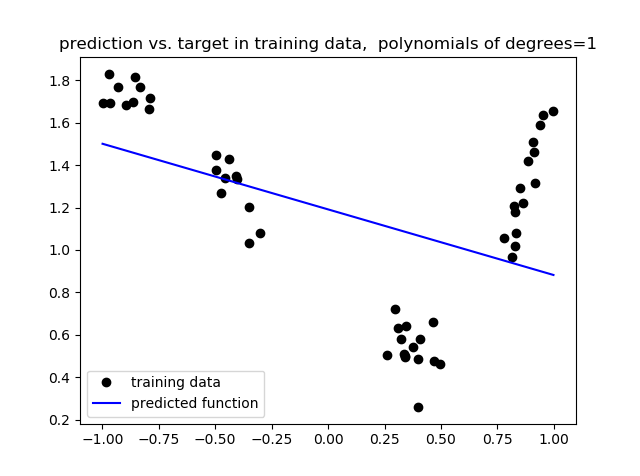
\includegraphics[width=0.5\textwidth]{Aufgabe_1a.png} 
\caption{Aufgabe1a } 
\label{Fig.main1}
\end{figure}
\end{subtask}
%-----------------------------------------------------------------------------------------------1b--------------------------------------------------------------------------------------------
\begin{subtask}[1b)]
Implement linear ridge regression using linear features, i.e. the data itself. Include an additional input dimension to
represent a bias term and use the ridge coefficient $ \mu = 0.01$.\\[15pt]
For polynomials of degrees 2, 3 and 4:\\
1. Report the root mean squared error of the training data and of the testing data under your model with polynomial
features. (2)\\[15pt]
2. Include a single plot that shows the training data as black dots and the predicted function as a blue line. (2)\\[15pt]
3. Why do we call this method linear regression despite using polynomials? (1)
\\[15pt]
answer:\\[15pt]
polynomials of degrees=1, root mean squared error of the training data: 1.4991687132735394\\
polynomials of degrees=1, root mean squared error of the training data: 2.1687242714148716\\
polynomials of degrees=2, root mean squared error of the training data: 0.6156652380614582\\
polynomials of degrees=2, root mean squared error of the training data: 1.0835803719738029\\
polynomials of degrees=3, root mean squared error of the training data: 0.6152720874799968\\
polynomials of degrees=3, root mean squared error of the training data: 1.0666239820964531\\
\begin{figure}[H] 
\centering 
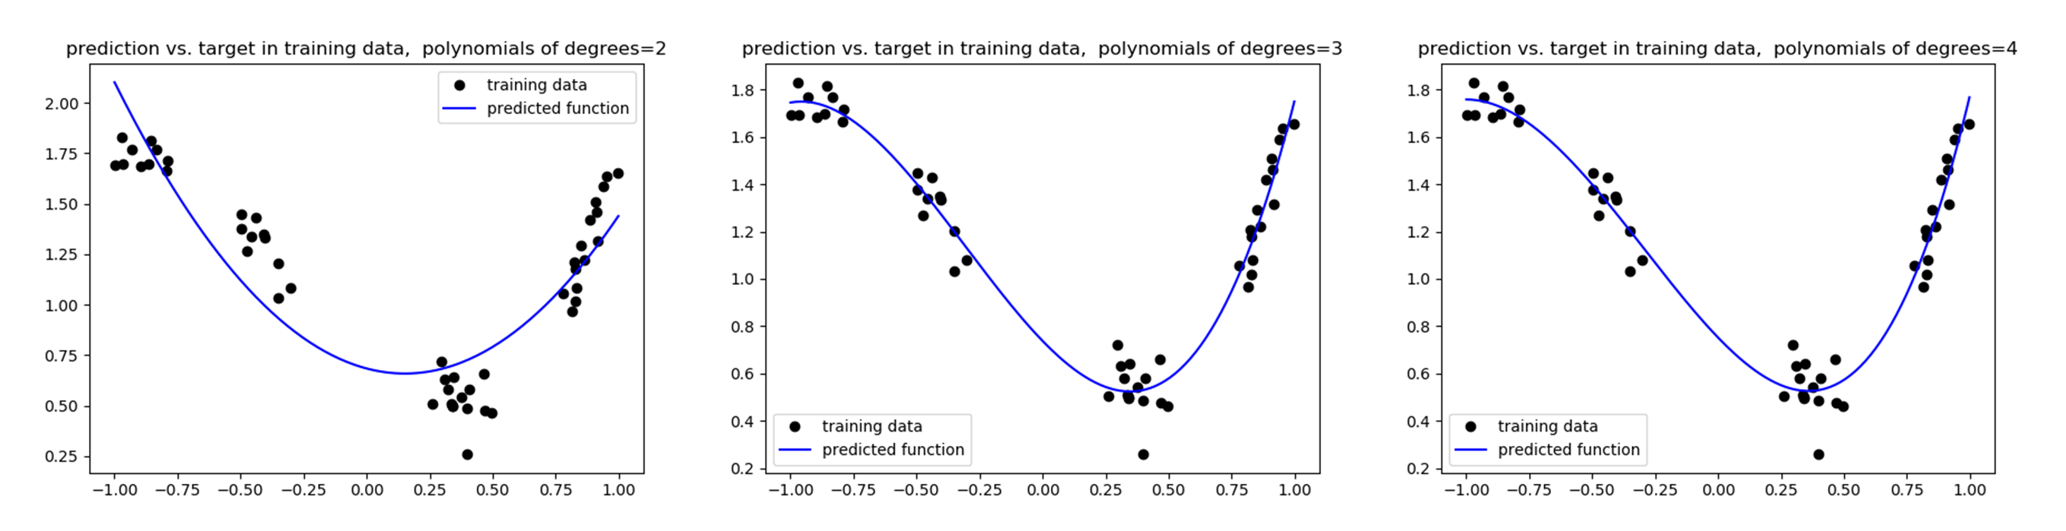
\includegraphics[width=1\textwidth]{Aufgabe_1b.png} 
\caption{Aufgabe1b } 
\label{Fig.main2}
\end{figure}
and the reason is $y_{pre} = \Phi_{hub}\cdot w$
\end{subtask}
%------------------------------------------------------------------------------------------------------1c---------------------------------------------------------------------------------------------------
\begin{subtask}[1c)]
Implement 5-fold cross-validation to select the optimal degree for your polynomial regression.\\
• Start by splitting the provided data into 5 distinct subsets with each subset consisting of 20\% of the original data.\\[15pt]
• Use subsets 1 - 4 to train your model with polynomial features of degrees 2, 3 and 4.\\[15pt]
• Compute the train RMSEs using your trained models and subsets 1 - 4.\\[15pt]
• Compute the validation RMSEs using your trained models and subset 5.\\[15pt]
• Compute the test RMSEs using your trained models and the test data.\\[15pt]
• Repeat the previous steps, cycling through the subsets until every subset has been used for validation.
Provide the following results and answers:\\[15pt]
1. For each polynomial degree, report the average train, validation and test RMSEs among all folds. (2)\\[15pt]
2. Explain: Do the resulting numbers meet your expectations? Why (not)? (2)\\[15pt]
3. Which polynomial degree should be chosen for the given data? Why? (1)
\\[15pt]
answer:\\[15pt]
polynomials of degrees=1, root mean squared error of training: 1.3246142423841534\\
polynomials of degrees=1, root mean squared error of validation: 0.7111489886262025\\
polynomials of degrees=1, root mean squared error of test: 2.183509401119271\\
polynomials of degrees=2, root mean squared error of training: 0.5452281414536173\\
polynomials of degrees=2, root mean squared error of validation: 0.2931779276868292\\
polynomials of degrees=2, root mean squared error of test: 1.092767157004997\\
polynomials of degrees=3, root mean squared error of training: 0.5405756570976916\\
polynomials of degrees=3, root mean squared error of validation: 0.3112176709628346\\
polynomials of degrees=3, root mean squared error of test: 1.0867173876433611\\

More polynomials of degrees $\rightarrow$ more precise prediction\\
Higher order polynomial could have more complex mapping, which can express more details of regression curve. But it could also lead to overfitting.\\
\[
\begin{array}{|l|l|l|}
\hline \text { polynomials of degrees } & \text { Mean of RMSE in Test } & \text { Std of RMSE in Test } \\
\hline 2 & 2.1835 & 0.08623 \\
\hline 3 & 1.0928 & 0.01533 \\
\hline 4 & 1.0867 & 0.02783 \\
\hline
\end{array}
\]
Chose polynomials of degrees 3 \\
Though 4-order polynomials has less Mean of RMSE in cross validation than 3 order, but it shows more Std of RMSE.
\end{subtask}
%----------------------------------------------------------------------------------------------------------1d----------------------------------------------------------------------------------------------
\begin{subtask}[1d)]
Implement Bayesian linear ridge regression, assuming that w follows a multivariate Gaussian distribution, such that
\[
\mathbf{w} \sim \mathcal{N}\left(\boldsymbol{\mu}_{0}, \boldsymbol{\Lambda}_{0}^{-1}\right)
\]
where ridge regression dictates $\mu_0 = 0$ and $\mathbf{\Lambda}_{0}=\lambda \mathbf{I} $\\
Here, $\mu_0$ is the prior weight mean and $\Lambda_0$ is the prior weight precision matrix, i.e. inverse of covariance matrix. The
corresponding posterior parameters can be denoted as $\mu_n$ and $\Lambda_n$.\\
Assume $\sigma = 0.1$, use $\lambda = 0.01$ and include an additional input dimension to represent a bias term. Use all of the
provided training data for a single Bayesian update.\\[15pt]
1. State the posterior distribution of the model parameters $p(\mathbf{w} \mid \mathbf{X}, \mathbf{y})$ (no derivation required). (1)\\[15pt]
2. State the predictive distributionp$\left(\mathbf{y}_{*} \mid \mathbf{X}_{*}, \mathbf{X}, \mathbf{y}\right)$ (no derivation required). (1)\\[15pt]
3. Report the RMSE of the train and test data under your Bayesian model (use the predictive mean). (1)\\[15pt]
4. Report the average log-likelihood of the train and test data under your Bayesian model. (1)\\[15pt]
5. Include a single plot that shows the training data as black dots, the mean of the predictive distribution as blue
line and 1, 2 and 3 standard deviations of the predictive distribution in shades of blue (you can use matplotlib’s
fill\_between function for that). (2)\\[15pt]
6. Explain the differences between linear regression and Bayesian linear regression. (1)
\\[15pt]
answer:\\[15pt]
1.
\[
\begin{aligned}
p(\mathbf{w} \mid \mathbf{X}, \mathbf{y}, \alpha, \beta) & \propto p(\mathbf{y} \mid \mathbf{X}, \mathbf{w}, \beta) p(\mathbf{w} \mid \alpha) \\
& \propto p(\mathbf{y} \mid \mathbf{X}, \mathbf{w}, \beta) \mathcal{N}\left(\mathbf{w} \mid \mathbf{0}, \alpha^{-1} \mathbf{l}\right)
\end{aligned}
\]
where 
$p(\mathbf{w} \mid \mathbf{X}, \mathbf{y}, \alpha, \beta)$ is the posterior
$p(\mathbf{y} \mid \mathbf{X}, \mathbf{w}, \beta) $ is the Likelihood of targets under the data and parameters
$p(\mathbf{w} \mid \alpha)$ is the prior\\[15pt]

2.
\[
p\left(y_{*} \mid \mathbf{x}_{*}, \mathbf{X}, \mathbf{y}\right)=\int \underbrace{p\left(y_{*} \mid \mathbf{x}_{*}, \theta\right)}_{\text {likelihood }} \underbrace{p(\theta \mid \mathbf{X}, \mathbf{y})}_{\text {parameter posterior }} \mathrm{d} \theta
\]
integrate out all possible parameters\\%-------------------------------------------------描述
RMSE of training data: 2.914538070997487 \\
RMSE of test data: 3.8433605616561968\\

average log-likelihood of training data: -1.5150672805423742\\
average log-likelihood of test data: -1.3940163553368101\\
\begin{figure}[H] 
\centering 
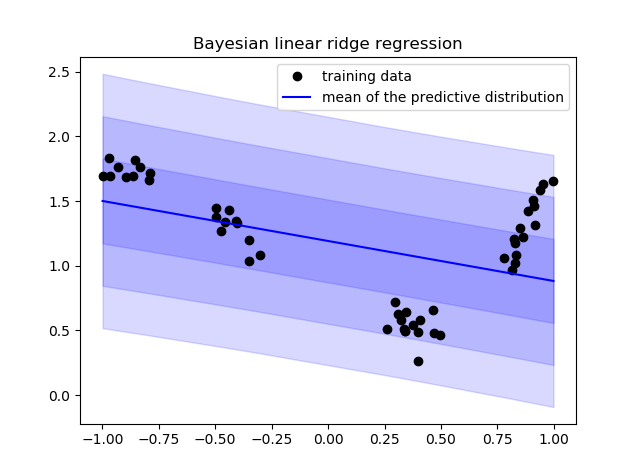
\includegraphics[width=0.5\textwidth]{Aufgabe_1d.png} 
\caption{Aufgabe1d } 
\label{Fig.main3}
\end{figure}
\end{subtask}
%---------------------------------------------------------------------------------------------------------1e--------------------------------------------------------------------------------------------
\begin{subtask}[1e)]
Implement Bayesian linear ridge regression using squared exponential (SE) features. In other words, replace your
observed data matrix $\mathrm{X} \in \mathbb{R}^{n \times 1}$, where:
\[
\Phi_{i j}=\exp \left(-\frac{1}{2} \beta\left(X_{i}-\alpha_{j}\right)^{2}\right) .
\]
Set $k = 20$, $\alpha_j = j \ast 0.1-1$ and  $\beta= 10$. Use the ridge coefficient $\lambda = 0.01$ and assume known Gaussian noise with
$\sigma = 0.1$. Include an additional input dimension to represent a bias term.\\
1. Report the RMSE of the train and test data under your Bayesian model with SE features. (1)\\[15pt]
2. Report the average log-likelihood of the train and test data under your Bayesian model with SE features. (1)\\[15pt]
3. Include a single plot that shows the training data as black dots, the mean of the predictive distribution as blue
line and 1, 2 and 3 standard deviations of the predictive distribution in shades of blue (you can use matplotlib’s
fill\_between function for that). (2)\\[15pt]
4. How can SE features be interpreted from a statisticians point of view? What are $\alpha$ and $\beta$ in that context? (2)\\[15pt]
\\[15pt]
answer:\\[15pt]
RMSE of training data: 0.5827509166240352\\
RMSE of test data: 1.1618310002287155\\
average log-likelihood of training data: -0.10392644293632658\\
average log-likelihood of test data: -0.22894630923741704\\

\begin{figure}[H] 
\centering 
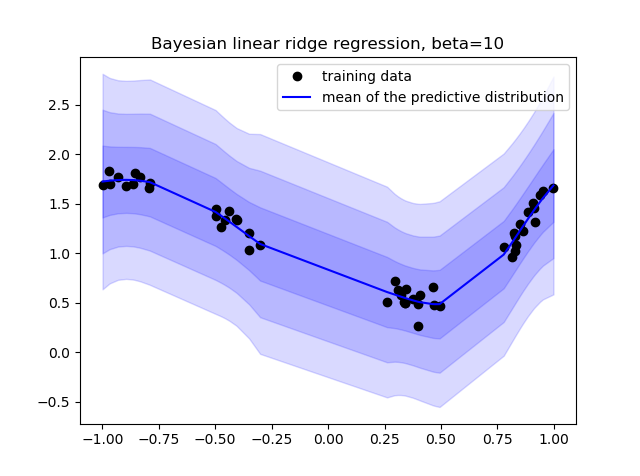
\includegraphics[width=0.5\textwidth]{Aufgabe_1e.png} 
\caption{Aufgabe1e } 
\label{Fig.main3}
\end{figure}

\end{subtask}
%-------------------------------------------------------------------------------------------------------1f-----------------------------------------------------------------------------------------------
\begin{subtask}[1f)]
In this bonus assignment, you will perform a grid search using  $\beta \in \{1,10,100\}$ to select a 'better' $\beta$ for your squared
exponential features from the previous subtask. Keep using the same settings as in the previous subtask, except $\beta$ .
Grid search is a simple method to select hyperparameters, such as$\beta$ . First, a list of possible values, or a grid, in case
of multiple hyperparameters, is created to define a discrete search space. For every value in this search space, a model
is trained and evaluated using a score or loss function. Finally, the hyperparameters that yield the highest score or
smallest loss are selected. Here, the log-marginal likelihood will be used as a score function.\\[15pt]
The log-marginal likelihood of our Bayesian linear model can be expressed as (see Bishop Ch. 3.5)
\[
\begin{aligned}
\log p(\mathbf{y} \mid \mathbf{X}) &=\log \int p(\mathbf{y} \mid \mathbf{X}, \mathbf{w}) p(\mathbf{w}) \mathrm{d} \mathbf{w},\\
&=\frac{k+1}{2} \log \lambda-\frac{n}{2} \log \sigma^{2}-\frac{1}{2} \frac{\|\mathbf{y}-\Phi \mu\|_{2}^{2}}{\sigma^{2}}+\frac{\lambda}{2} \mu^{\top} \mu-\frac{1}{2} \log |\mathbf{\Lambda}|-\frac{n}{2} \log 2 \pi
\end{aligned}
\]
where
\[
\begin{aligned}
\boldsymbol{\mu}&=\sigma^{-2} \boldsymbol{\Lambda}^{-1} \boldsymbol{\Phi}^{\top} \mathbf{y} \\
\boldsymbol{\Lambda}&=\sigma^{-2} \boldsymbol{\Phi}^{\top} \boldsymbol{\Phi}+\lambda \mathbf{I}
\end{aligned}
\]
\\[15pt]
Here, $k$ is the dimensionality of the feature space, the $+1$ comes from the extra bias term.
Using the marginal likelihood to select hyperparameters is typically referred to as empirical Bayes, type-II maximum
likelihood or evidence approximation. Applying the logarithm (analytically) ensures numerical stability.\\[15pt]
1. What is the difference between the marginal likelihood $p(y| X)$ and the likelihood $p(y | X, w)$? (1) \\[15pt]
2. For each $\beta$, report RMSE and average log-likelihood of the train and test data and the log-marginal likelihood.
(3)\\[15pt]
3. For each beta, include a single plot that shows the training data as black dots, the mean of the predictive distribution
as blue line and 1, 2 and 3 standard deviations of the predictive distribution in shades of blue (you can use
matplotlib's fill\_between function for that). (2)\\[15pt]
4. According to the grid search, which value for $\beta$is the best? Why? (2)\\[15pt]
5. Compare the log-marginal likelihood values to the average train and test log-likelihood values. What do you
observe? Is the log-marginal likelihood a ‘good’ score function compared to the train log-likelihood? (2)\\
answer:\\[15pt]
\[
\begin{array}{|c|c|c|c|}
\hline \mathrm{SE} & 1 & 10 & 100 \\
\hline \text { RMSE of training data } & 0.9174 & 0.5828 & 0.5498 \\
\hline \begin{array}{c}
\text { average log-likelihood } \\
\text { of training data }
\end{array} & -0.2917 & -0.1039 & -0.0856 \\
\hline \text { RMSE of test data } & 1.5690 & 1.1618 & 1.6271 \\
\hline \begin{array}{c}
\text { average log-likelihood } \\
\text { of test data }
\end{array} & -0.3976 & -0.2289 & -0.3902 \\
\hline \begin{array}{c}
\text { log-marginal likelihood } \\
\text { of training data }
\end{array} & -22.3919 & 1.1271 & 3.3718 \\
\hline \begin{array}{c}
\text { log-marginal likelihood } \\
\text { of test data }
\end{array} & -103.3937 & -49.3719 & -112.0934 \\
\hline
\end{array}
\]
\begin{figure}[H] 
\centering 
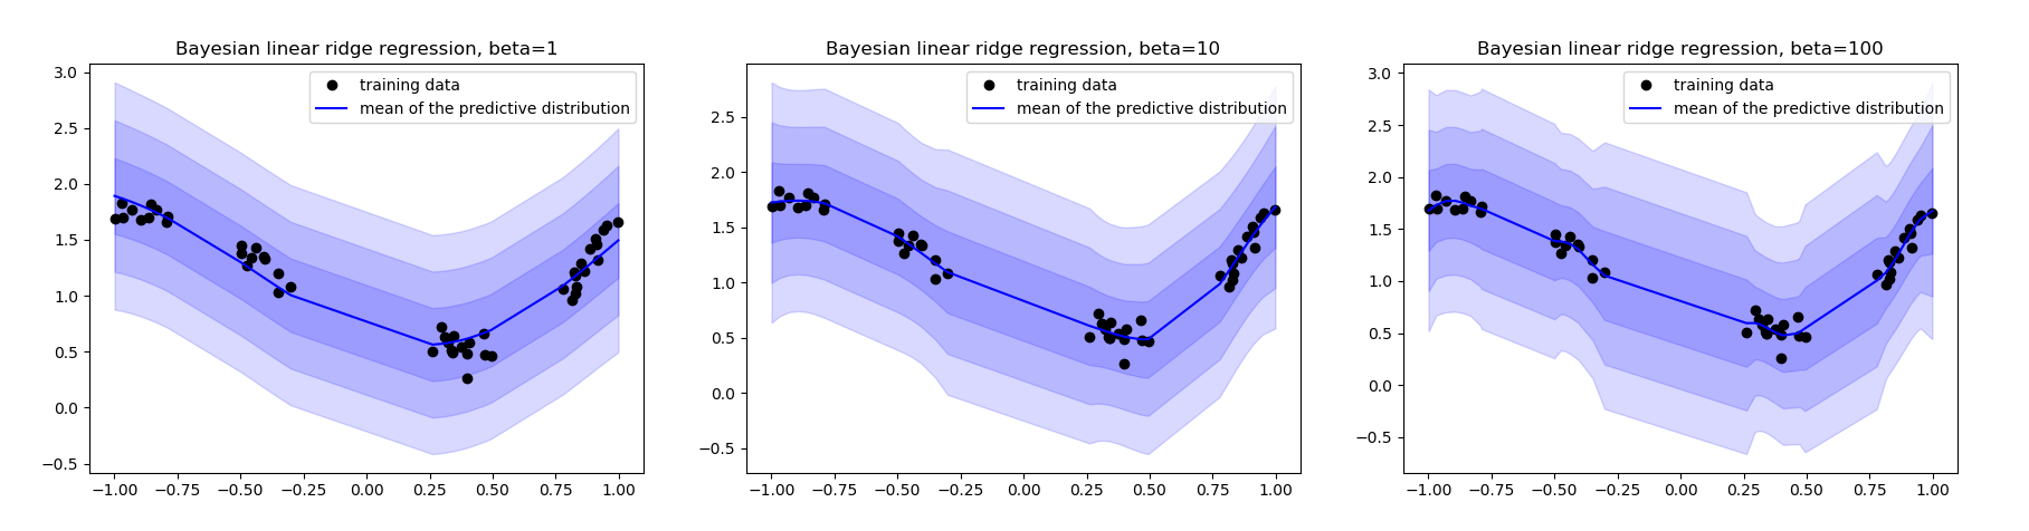
\includegraphics[width=1\textwidth]{Aufgabe_1f.png} 
\caption{Aufgabe1f } 
\label{Fig.main3}
\end{figure}
according to RMSE in Test, best beta is 100 \\
according to log-likelihood in Test, best beta is 10 \\
according to log-marginal likelihood in Test, best beta is 10 \\
Although beta = 100 performs best in RMSE, its variance is significantly larger. Based on the results of log-likelihood and log-marginal likelihood, the best beta should be 10 \\

Log-marginal likelihood includes consideration of the weight matrix mue and ridge coefficient.\\
In terms of loss function (ie, score function), the occurrence of overfitting can be reduced to a certain extent.\\
\end{subtask}
\end{task}
\newpage
%-------------------------------------------------------------------------------------------------------Task2--------------------------------------------------------------------------------------------
\begin{task}{Linear Classification}
In this exercise, you will use the dataset ldaData.txt, , containing 137 feature points $\vec{x}$. The first 50 points belong to
class $C_1$, the second 43 to class $C_2$, the last 44 to class $C_3$.
%-----------------------------------------------------------------------------------------------------------2a-------------------------------------------------------------------------------------------
\begin{subtask}[2a)]
Explain the difference between discriminative and generative models and give an example for each case. Which model
category is generally easier to learn and why?\\
Answer:\\[15pt]
In General, A Discriminative model ‌models the decision boundary between the classes. A Generative Model ‌explicitly models the actual distribution of each class. \\[15pt]
A Generative Model ‌learns the joint probability distribution $p(x,y)$. It predicts the conditional probability with the help of Bayes Theorem. A Discriminative model ‌learns the conditional probability distribution $p(y|x)$. Both of these models were generally used in supervised learning problems.\\[15pt]
In general generative models are easier to learn than discriminative models. Because in practice, it  is usually
hard to compte the postrior for discriminative models.

\end{subtask}
\newpage
%---------------------------------------------------------------------------------------------------2b-------------------------------------------------------------------------------------------------
\begin{subtask}[2b)]
Use Linear Discriminant Analysis to classify the points in the dataset. Attach two plots with the data points using a
different color for each class: one plot with the original dataset, one with the samples classified according to your LDA
classifier. Attach a snippet of your code and discuss the results. How many samples are misclassified? (You are allowed
to use built-in functions for computing the mean and the covariance.)
\\[15pt]
answer:\\[15pt]
\begin{lstlisting}
# -*- coding: utf-8 -*-

import numpy as np
import matplotlib.pyplot as plt

def load_data(filename):
    data = np.loadtxt(f"D:\\Test\\dataSets\\{filename}.txt")
    C_1 = np.mat(data[:50, :]).T
    C_2 = np.mat(data[50:93,:]).T
    C_3 = np.mat(data[93:, :]).T
    return C_1, C_2 ,C_3, data

def normal_vec_w (c_1,c_2):
    mean_c_1 = np.mean(c_1,1)
    mean_c_2 = np.mean(c_2,1)
    diff_w = np.dot ((c_1 - mean_c_1), ((c_1 - mean_c_1).T)) + np.dot ((c_2 - mean_c_2), ((c_2 - mean_c_2).T))
    mat_w = np.dot(np.linalg.inv(diff_w), (mean_c_2 - mean_c_1)) 
    normal_w = mat_w[0] / mat_w[1]
    return mat_w, normal_w

def offset(w, c_1, c_2):
    c1_re = np.dot(w.T , c_1)
    c2_re = np.dot(w.T , c_2)
    mean_c1_re = np.mean(c1_re)
    mean_c2_re = np.mean(c2_re)
    var_c1_re = np.var(c1_re)
    var_c2_re = np.var(c2_re)
    r1 = 1 / (2 * var_c1_re) - 1 / (2 * var_c2_re)
    r2 = (mean_c2_re / var_c2_re) - (mean_c1_re / var_c1_re)
    r3 = mean_c1_re ** 2 / (2 * var_c1_re) - mean_c2_re ** 2 / (2 * var_c2_re) - np.log(np.sqrt(var_c2_re/var_c1_re))
    
    root_r = np.roots([r1, r2, r3])
    for i in range (len(root_r)):
        if root_r[i] < max(mean_c1_re, mean_c2_re) and root_r[i] > min(mean_c1_re , mean_c2_re):
            w0 = root_r[i]
            break 
    return w0

if __name__ == "__main__":
    C_1, C_2, C_3, data = load_data('ldaData')
    a = C_1.T
    b = C_2.T
    c = C_3.T
    
    mat_w12, normal_w12 = normal_vec_w(C_1,C_2)
    mat_w13, normal_w13 = normal_vec_w(C_1,C_3)
    mat_w23, normal_w23 = normal_vec_w(C_2,C_3)
    
    w0_12 = offset(mat_w12,C_1, C_2)
    w0_13 = offset(mat_w13,C_1, C_3)
    w0_23 = offset(mat_w23,C_2, C_3)
    
    #without LDF
    for i in range(len(a)):
        plt.scatter(a[i, 0], a[i, 1] , marker = 'v' , color = 'red')
        i = i + 1
        
    for i in range(len(b)):
        plt.scatter(b[i, 0], b[i, 1] , marker = 'x' , color = 'yellow')
        i = i + 1
        
    for i in range(len(c)):
        plt.scatter(c[i, 0], c[i, 1] , marker = 'o' , color = 'blue')
        i = i + 1
        
    plt.show()

    # with LDF
    for i in range(len( data )):
        if np.dot(mat_w12.T, np.mat(data[i, :]).T) - w0_12 < 0:
            plt.scatter(data[i, 0], data[i, 1] , marker = 'v' , color = 'red')
        elif np.dot(mat_w23.T, np.mat(data[i, :]).T) - w0_23 < 0:
            plt.scatter(data[i, 0], data[i, 1], marker = 'x', color = 'yellow')
        else:
            plt.scatter(data[i, 0], data[i, 1], marker = 'o', color = 'blue')
        i = i + 1
    plt.show()
\end{lstlisting}
\begin{figure}[H] 
\centering 
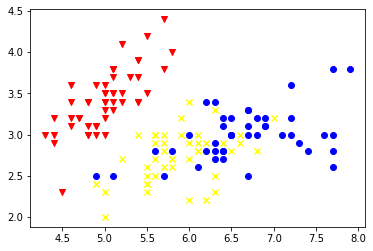
\includegraphics[width=0.5\textwidth]{Aufgabe_2b1.png} 
\caption{Aufgabe2b\_original\_classes } 
\label{Fig.main3}
\end{figure}
\begin{figure}[H] 
\centering 
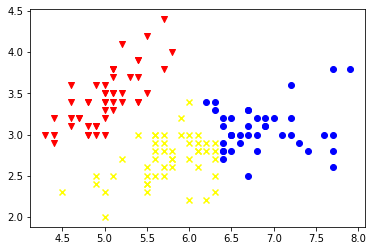
\includegraphics[width=0.5\textwidth]{Aufgabe_2b2.png} 
\caption{Aufgabe2b\_classes\_with\_LDA } 
\label{Fig.main3}
\end{figure}
\end{subtask}

\end{task}
\newpage
%----------------------------------------------------------------------------------3-----------------------------------------------------------------
\begin{task}{Principal Component Analysis}
In this exercise, you will use the dataset iris.txt. It contains data from three kind of Iris flowers (‘Setosa’, ‘Versicolour’
and ‘Virginica’) with 4 attributes: sepal length, sepal width, petal length, and petal width. Each row contains a sample
while the last attribute is the label (0 means that the sample comes from a ‘Setosa’ plant, 1 from a ‘Versicolour’ and
2 from ‘Virginica’). (You are allowed to use built-in functions for computing the mean, the covariance, eigenvalues,
eigenvectors and singular value decomposition.)
%--------------------------------------------------------------------------------------------------------3a-----------------------------------------
\begin{subtask}[3a)]
Normalizing the data is a common practice in machine learning. Normalize the provided dataset such that it has zero
mean and unit variance per dimension. Why is normalizing important? Attach a snippet of your code.\\[15pt]
answer:\\[15pt]
Normalization is important in PCA since it is a variance maximizing exercise. It projects the original data onto directions which maximize the variance.\\
And it will give more emphasis to those variables having higher variances than to those variables with very low variances while identifying the right principle component.
\begin{lstlisting}
def normalization(dataset):
    x , y = np.shape(dataset)
    for i in range( y - 1):
        dataset[: , i] = dataset[: , i] - np.mean(dataset[: , i])
        dataset[: , i] = dataset[: ,i] * np.sqrt(x / float(np.dot(np.mat(dataset[: , i]), np.mat(dataset[: , i]).T)))
        return x, y, dataset
\end{lstlisting}
\end{subtask}
%--------------------------------------------------------------------------------------------------------------3b-----------------------------------
\begin{subtask}[3b)]
Apply PCA on your normalized dataset and generate a plot showing the proportion (percentage) of the cumulative
variance explained. How many components do you need in order to explain at least 95\% of the dataset variance?
Attach a snippet of your code.\\[15pt]
answer:\\[15pt]
\begin{lstlisting}

# -*- coding: utf-8 -*-

import numpy as np
import matplotlib.pyplot as plt

def load_data(filename):
    data = np.loadtxt(f"D:\\Test\\dataSets\\{filename}.txt" , delimiter = ',')
    return data

def normalization(dataset):
    x , y = np.shape(dataset)
    for i in range( y - 1):
        dataset[: , i] = dataset[: , i] - np.mean(dataset[: , i])
        dataset[: , i] = dataset[: ,i] * np.sqrt(x / float(np.dot(np.mat(dataset[: , i]), np.mat(dataset[: , i]).T)))
        return x, y, dataset
    
if __name__ == "__main__":
    data_raw = load_data('iris')
    N, M, data_norm = normalization(data_raw)
    
    data_cal = np.mat(data_norm[: , 0 : 4]).T
    cov_data = np.cov(data_cal)
    lambda_data , W = np.linalg.eig(cov_data)
    
    #3b
    lambda_norm = lambda_data / np.sum(lambda_data)
    a = np.linspace(1, M-1, M-1)
    b = np.zeros(M-1)
    for i in range(M-1):
        b[i] = np.sum(lambda_norm[: i+1])
    plt.plot(a, b)
    plt.show()
\end{lstlisting}
\begin{figure}[H] 
\centering 
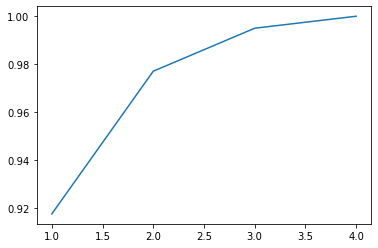
\includegraphics[width=0.5\textwidth]{Aufgabe3_b.png} 
\caption{Aufgabe3b} 
\label{Fig.main3}
\end{figure}
the two first varicance are needed, to explain at least 95\% of the dataset variance, as it is seen in the picture.
\end{subtask}
%----------------------------------------------------------------------------------------3c-------------------------------------------------------
\begin{subtask}[3c)]
Using as many components as needed to explain 95\% of the dataset variance, generate a scatter plot of the lowerdimensional
projection of the data. Use different colors or symbols for data points from different classes. What do you
observe? Attach a snippet of your code.\\[15pt]
answer:\\[15pt]
\begin{lstlisting}
# -*- coding: utf-8 -*-

import numpy as np
import matplotlib.pyplot as plt

def load_data(filename):
    data = np.loadtxt(f"D:\\Test\\dataSets\\{filename}.txt" , delimiter = ',')
    return data

def normalization(dataset):
    x , y = np.shape(dataset)
    for i in range( y - 1):
        dataset[: , i] = dataset[: , i] - np.mean(dataset[: , i])
        dataset[: , i] = dataset[: ,i] * np.sqrt(x / float(np.dot(np.mat(dataset[: , i]), np.mat(dataset[: , i]).T)))
        return x, y, dataset

if __name__ == "__main__":
    data_raw = load_data('iris')
    N, M, data_norm = normalization(data_raw)
    
    data_cal = np.mat(data_norm[: , 0 : 4]).T
    cov_data = np.cov(data_cal)
    lambda_data , W = np.linalg.eig(cov_data)

    #3c
    B = np.mat(W[: , 0: 2]) 
    class_2d = np.dot(B.T, (data_cal - np.mean(data_cal, 1)))
    for i in range(N):
        if data_norm[i, 4] == 0:
            plt.scatter (class_2d[0 , i], class_2d[1 , i], marker = 'v', color = 'red')
        elif data_norm[i, 4] == 1:
            plt.scatter (class_2d[0 , i], class_2d[1 , i], marker = 'x', color = 'yellow')
        else:
            plt.scatter (class_2d[0 , i], class_2d[1 , i], marker = 'o', color = 'blue')
    plt.show()
\end{lstlisting}
\begin{figure}[H] 
\centering 
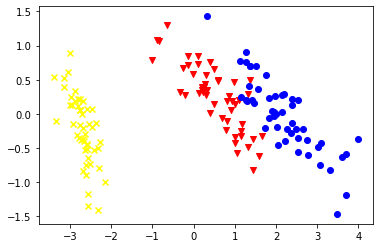
\includegraphics[width=0.5\textwidth]{Aufgabe3_c.png} 
\caption{Aufgabe3c} 
\label{Fig.main3}
\end{figure}
\end{subtask}
%-----------------------------------------------------------------------------------------------------3d----------------------------------------------
\begin{subtask}[3d)]
Reconstruct the original dataset by using different number of principal components. Using the normalized root mean
square error (NRMSE) as a metric, fill the table below (error per input versus the amount of principal components used).\\[15pt]
answer:\\[15pt]
\[
\begin{array}{c|c|c|c|c}
\text { N. of components } & x_{1} & x_{2} & x_{3} & x_{4} \\
\hline 1 & & & & \\
2 & & & & \\
3 & & & & \\
4 & & & &
\end{array}
\]
Attach a snippet of your code. (Remember that in the first step you normalized the data.)\\[15pt]
answer:\\[15pt]
\begin{lstlisting}
# -*- coding: utf-8 -*-

import numpy as np
import matplotlib.pyplot as plt

def load_data(filename):
    data = np.loadtxt(f"D:\\Test\\dataSets\\{filename}.txt" , delimiter = ',')
    return data

if __name__ == "__main__":
    data_raw = load_data('iris')
    #3d
    data_cal_raw = np.mat(data_raw[: , 0 : 4]).T
    error = np.mat(np.zeros((4,4)))
    cov_data_raw = np.cov(data_cal_raw)
    lambda_data_raw , W_raw = np.linalg.eig(cov_data_raw)
    for i in range(M - 1):
        B_raw = np.mat(W_raw[:, 0: i+1])
        class_2d_raw = np.dot(B_raw.T, (data_cal_raw - np.mean(data_cal_raw, 1)))
        datau_cal = np.mean(data_cal_raw, 1) + np.dot(B_raw ,class_2d_raw)
        error[i, :] = np.sqrt(np.sum(np.power((data_cal_raw - datau_cal), 2), 1) / N).T
    print(error)
\end{lstlisting}
As a result the table will be filled:
\[
\begin{array}{c|c|c|c|c}
\text { N. of components } & x_{1} & x_{2} & x_{3} & x_{4} \\
\hline 1 & 0.4137& 0.4010 & 0.1615 & 0.2058\\
2 & 0.1485 & 0.2131 & 0.0813 & 0.1929 \\
3 & 0.0389& 0.0496 & 0.0753&  0.1209\\
4 & 0& 0& 0&0
\end{array}
\]
\end{subtask}
%-----------------------------------------------------------------------------------------------3e------------------------------------------------------
\begin{subtask}[3e)]
In machine learning, it is often desirable to ‘whiten’ the data before applying a model or an algorithm. In this context,
‘whitening’ the data refers to a transformation that warps the data into a spherical shape, such that the data dimensions
become uncorrelated and the individual means and variances are 0 and 1, respectively. In particular, PCA can be used
to compute such a transformation.\\
Recommended reading: ufldl.stanford.edu/tutorial/unsupervised/PCAWhitening\\[15pt]
1. Explain the difference between PCA and ZCA whitening. (1)\\[15pt]
2. State the equation(s) to compute the ZCA whitening parameters, given the data. (1)\\[15pt]
3. State the equation(s) to whiten a (new) data example x, given the ZCA parameters. (1)\\[15pt]
4. Compute and report the ZCA whitening parameters for the unnormalized IRIS data (including numerical values!).\\
For numerical stability, use $\epsilon=1 e-5$ (2)\\[15pt]
answer:\\[15pt]
1.For PCA whiting , the Covariance is exact 1, and for ZCA whiting , the Covariance is same but not strict 1.
And PCA wihting can be done to reduce the demension, while ZCA is more used to uncorrelate.\\
2.
\[
X_{\text {ZCAwhiting}}=U X_{\text {PCAWhite}, i}
\]
3.
\[
\begin{aligned}
\Sigma &= \frac{1}{m} X X^{T}\\
\frac{1}{m} X X^{T} &=U A U^{T}\\
X_{r o t}&=U^{T} X \\
X_{\text {PCAwhite }, i} & =\frac{X_{\text {rot }, i}}{\sqrt{\lambda_{i}+e}}, e=1.0 e^{-5}\\
X_{\text {ZCAwhiting}}&=U X_{\text {PCAWhite}, i}
\end{aligned}
\]
\end{subtask}
%--------------------------------------------------------------------------------------3f------------------------------------------------------
\begin{subtask}[3f)]
Throughout this class we have seen that PCA is an easy and efficient way to reduce the dimensionality of
some data. However, it is able to detect only linear dependences among data points. A more sophisticated
extension to PCA, Kernel PCA, is able to overcome this limitation. This question asks you to deepen this topic
by conducting some research by yourself: explain what Kernel PCA is, how it works and what are its main
limitations. Be as concise (but clear) as possible.\\[15pt]
answer:\\[15pt]
Kernel PCA: an extension of principal component analysis (PCA) using techniques of kernel methods. Using a kernel, the originally linear operations of PCA are performed in a reproducing kernel Hilbert space.\\
Process: Solve the following eigenvalue problem:\\
\[
K u_{i}=\lambda_{i} u_{i}, \lambda_{1} \geq \lambda_{2} \geq \ldots \geq \lambda_{N}
\]
The projection of the test sample $\Phi (X_j)$ on the i\_th eigenvector can be computed by
\[
K u_{i}=\lambda_{i} u_{i}, \lambda_{1} \geq \lambda_{2} \geq \ldots \geq \lambda_{N}v_{i}^{T} \Phi\left(x_{j}\right)=\frac{1}{\sqrt{\lambda_{j}}} u_{i}^{T}\left[\begin{array}{c}
K\left(x_{1}, x_{j}\right) \\
\vdots \\
K\left(x_{N}, x_{j}\right)
\end{array}\right]
\]
limitations:\\
a) PCA assumes a linear transformation: $\rightarrow$ With centering of data, one can only do a rotation in space. \\
b) It fails at finding directions that require a non-linear transformation. \\
\end{subtask}
\end{task}
\end{document}
